% MDW: I have moved this to a separate file since I don't know yet
% where it should go.

%  - xcorr with Node 213 and Reftek data [GWA]
%    - Relate to timing confidence: Are events with good FTSP timing 
%      more accurate?

\subsection{Comparison with broadband station}
\label{sec-datagroundtruthing}

\begin{figure}[t]
\begin{center}
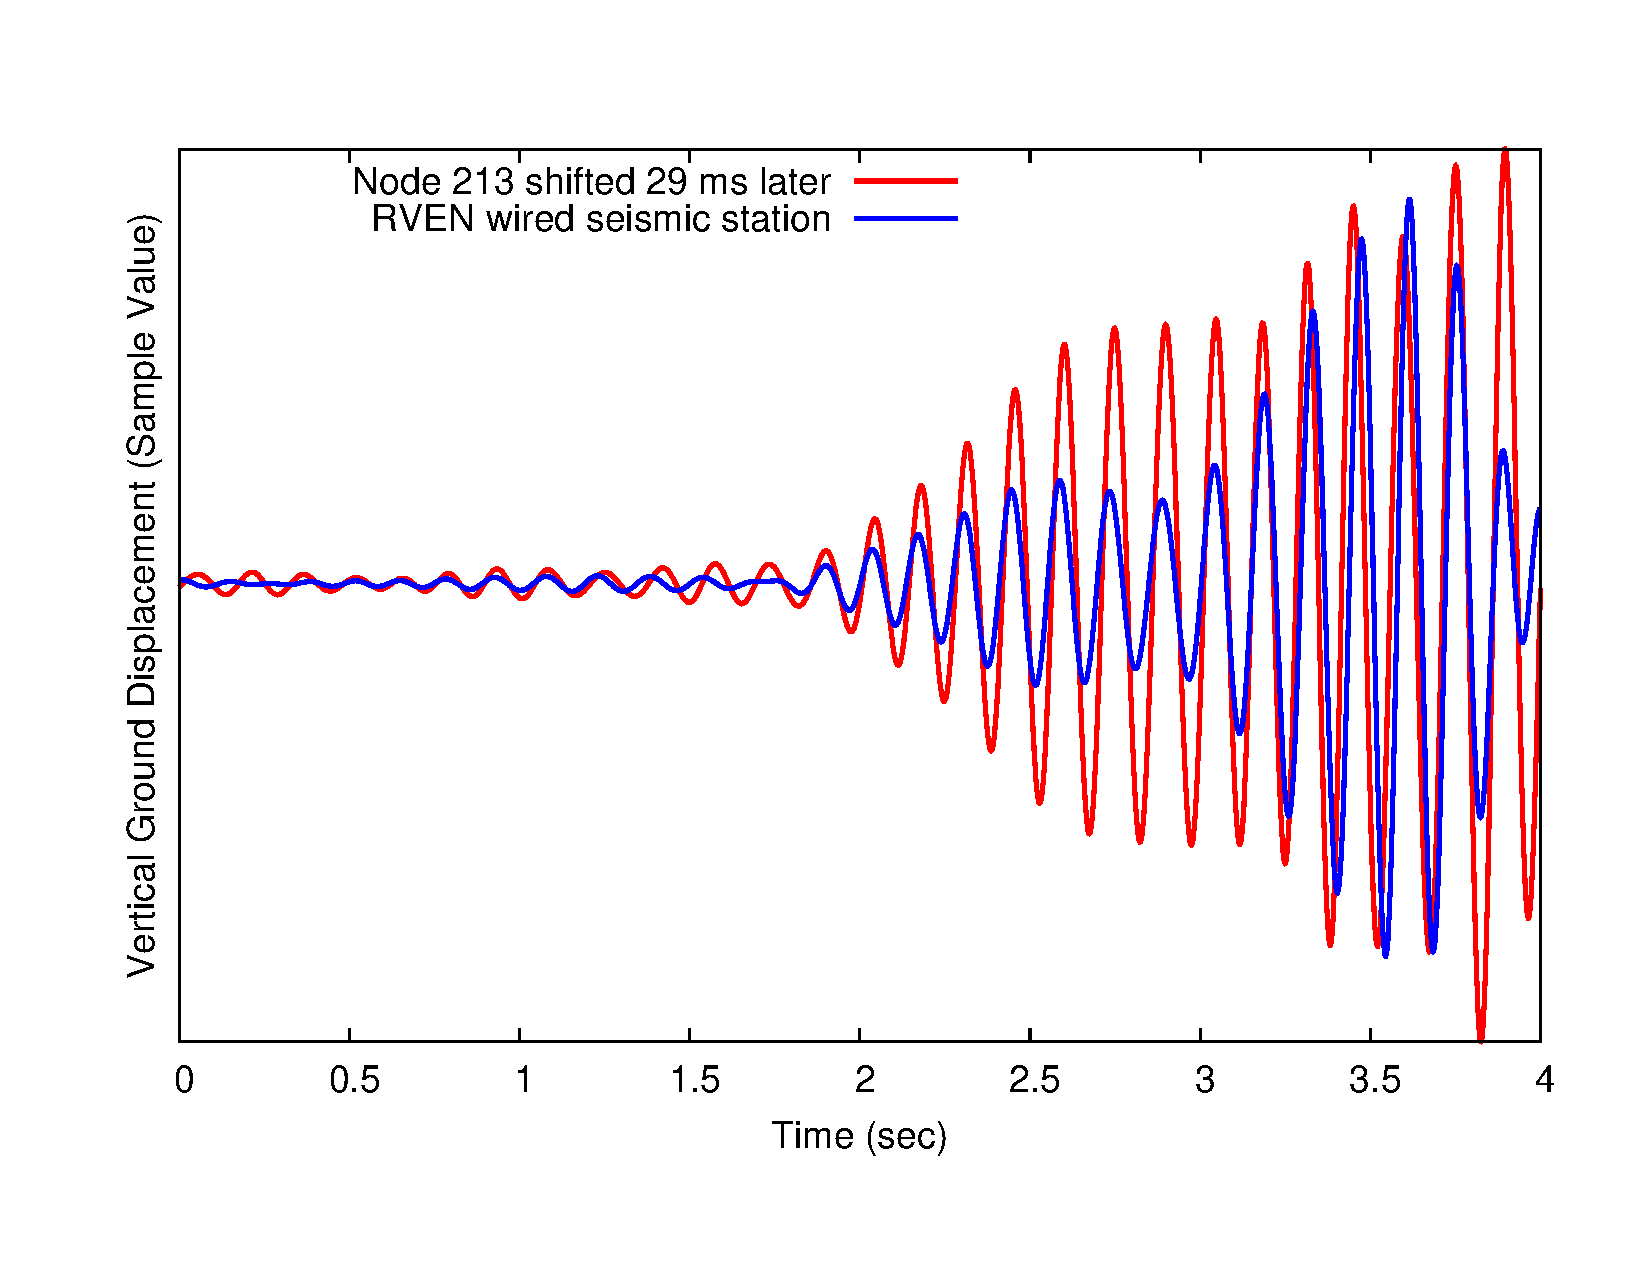
\includegraphics[width=\hsize]{./casestudy/figs/timing/ReftekV213/2005-08-15_09.11.28/213VREFTEK-NEGATIVE29MS-OFFSET.pdf}
\end{center}
\caption{\small {\bf Comparison of RVEN and node~213 signals.} 
{\em This figure shows two seismic waves recorded by sensor node 213 and a
broadband seismometer located 56~m away. After time rectification, a 29~ms
time shift produces an excellent match.}}
\label{fig-rvenv213}
\end{figure}

Although time rectification works well in the laboratory, it is also
necessary to evaluate its accuracy on the data collected during the field
deployment. For this purpose, we made use of one of the broadband seismometer
stations colocated with our sensor network. The RVEN (for ``Reventador
vent'') station was located 56~m from sensor node~213.  
Given their proximity, we would expect
the seismic waveforms captured by both RVEN and node~213 to be
well correlated.  Some time shift between the two signals would be expected:
a seismic wave passing each station could be as slow as 1.5~km/sec, so
the time lag between the signals could be as high as 37~ms.  However, due to
differences in the seismometers and the placement and ground coupling of the
sensors, we would not expect perfectly correlated signals in every
case.

% MDW: Not sure this is really needed.
%As a first step we collected the sample rates calculated as the last step in
%the time rectification process.  Since the sampling rate was driven by a
%separate oscillator on the sensor interface board we can use its expected
%sample rate as another check that the time rectified data makes sense.
%Indeed we find that 94\% of time-rectified data records report sample rates
%within the manufacturing tolerances of the 10~MHz, 50 PPM interface board
%oscillator.

We identified 28~events recorded by both RVEN and node~213.  The data for
node~213 was time rectified as described earlier, and the RVEN data was
timestamped by the Reftek's internal GPS receiver.  We applied a bandpass
filter of 6--8~Hz to each signal to reduce sensor-specific artifacts. The
cross-correlation between the signals produces a set of
of {\em lag times} indicating possible time shifts between the two signals.
Due to the periodic nature of the signals, this results in
several lag times at multiples of the dominant signal period. For each lag
time, we visually inspected how well the time-shifted signals overlapped and
picked the best match by hand.


\begin{figure}[t]
\begin{center}
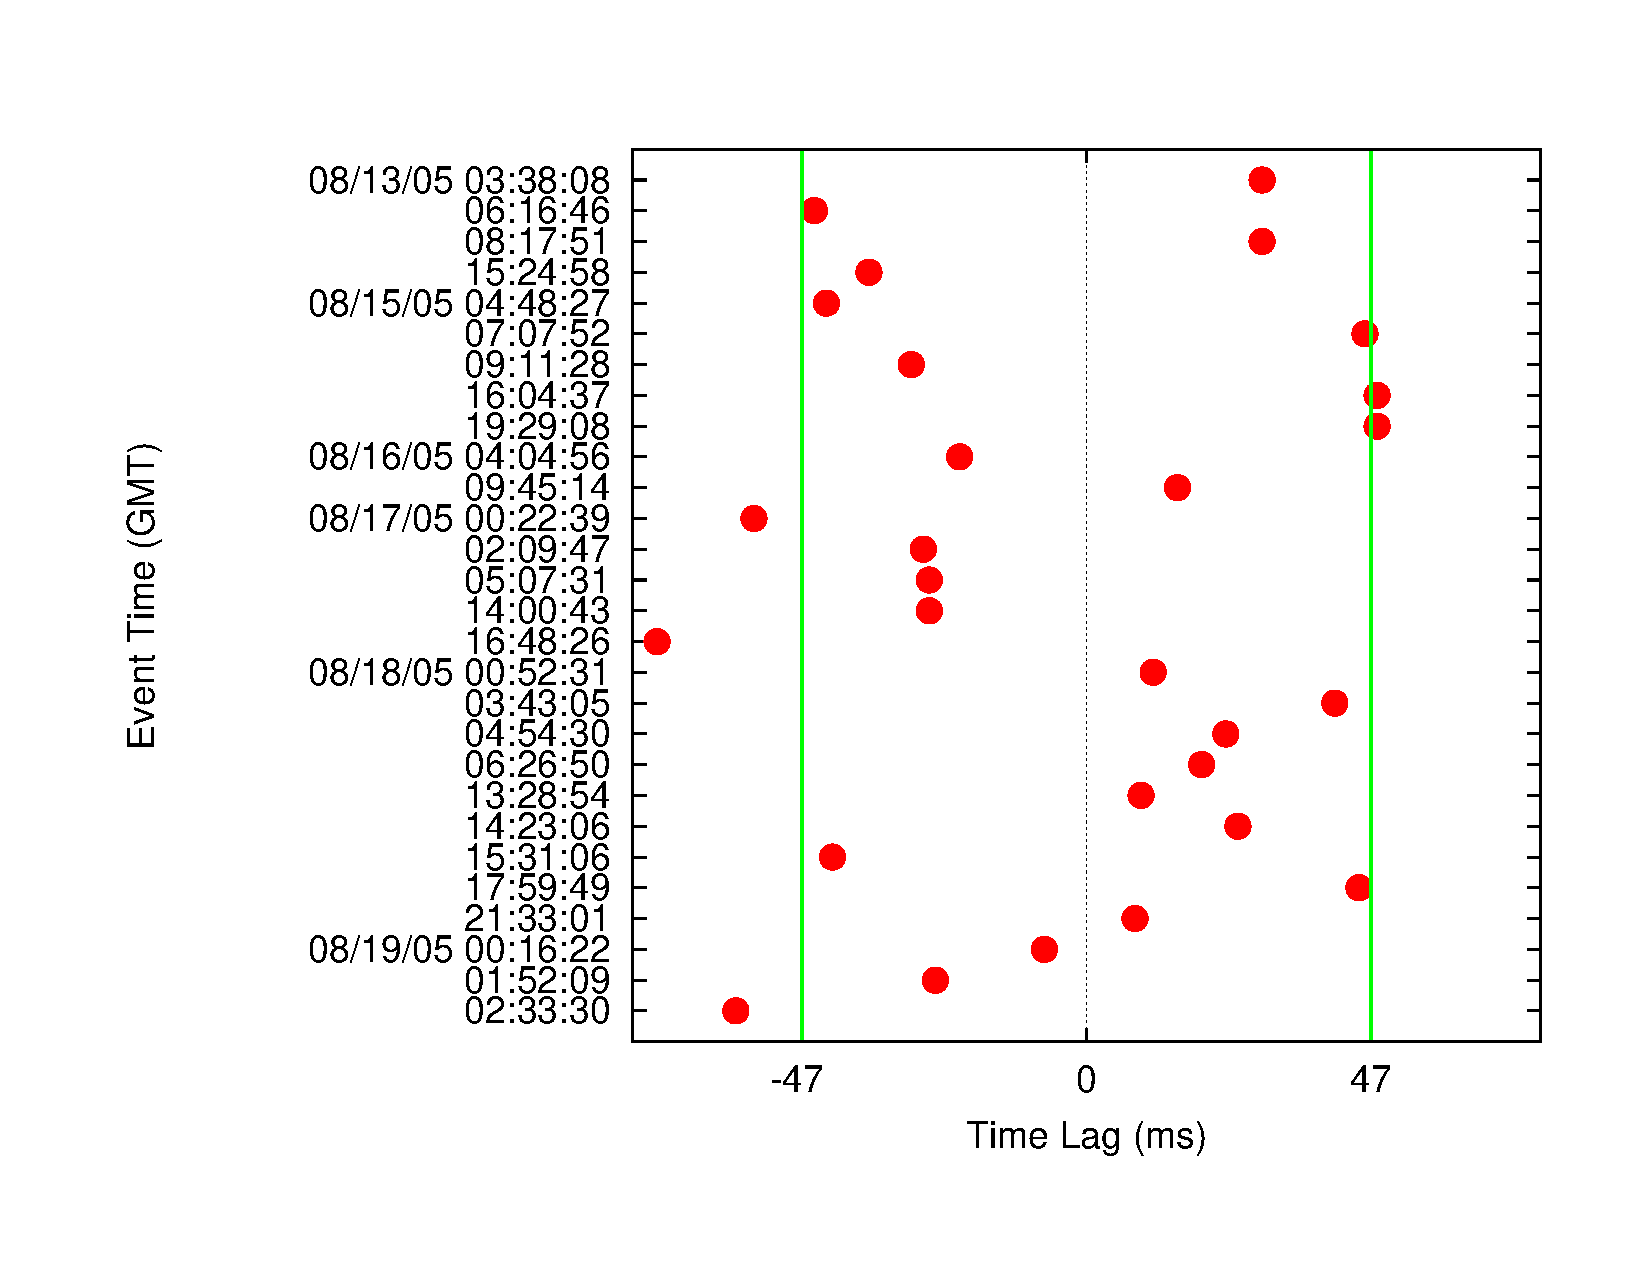
\includegraphics[width=\hsize]{./casestudy/figs/timing/ReftekV213/Table/213-GOODDIFFS2.pdf}
\end{center}
\caption{\small{\bf Lag times between Node 213 and RVEN.}
{\em The best lag time between the two stations is shown for 28 events.  best
time lag between the two stations is shown.  Most time shifts into the
+/-~47~ms window that we would expect given the distance between the two
stations and up to 10~ms of timing error.}}
\label{fig-rvenv213all}
\end{figure}

Figure~\ref{fig-rvenv213} shows an example of this process that demonstrates
excellent correlation between the RVEN and node~213 signals with a 29~ms time
shift. Figure~\ref{fig-rvenv213all} shows a scatterplot of the best lag times
for all~28~events.  Of these, only 5~events fall outside of a $+/-$~47~ms
window defined by the distance between the stations ($+/-$~37~ms) and our
acceptable sampling error (10~ms). We have high confidence that our
time rectification process was able to recover accurate timing despite
failures of the FTSP protocol.
%This demonstrates that the time
%rectification process was able to recover accurate timing for these signals.

%\begin{figure}[t]
%\begin{center}
%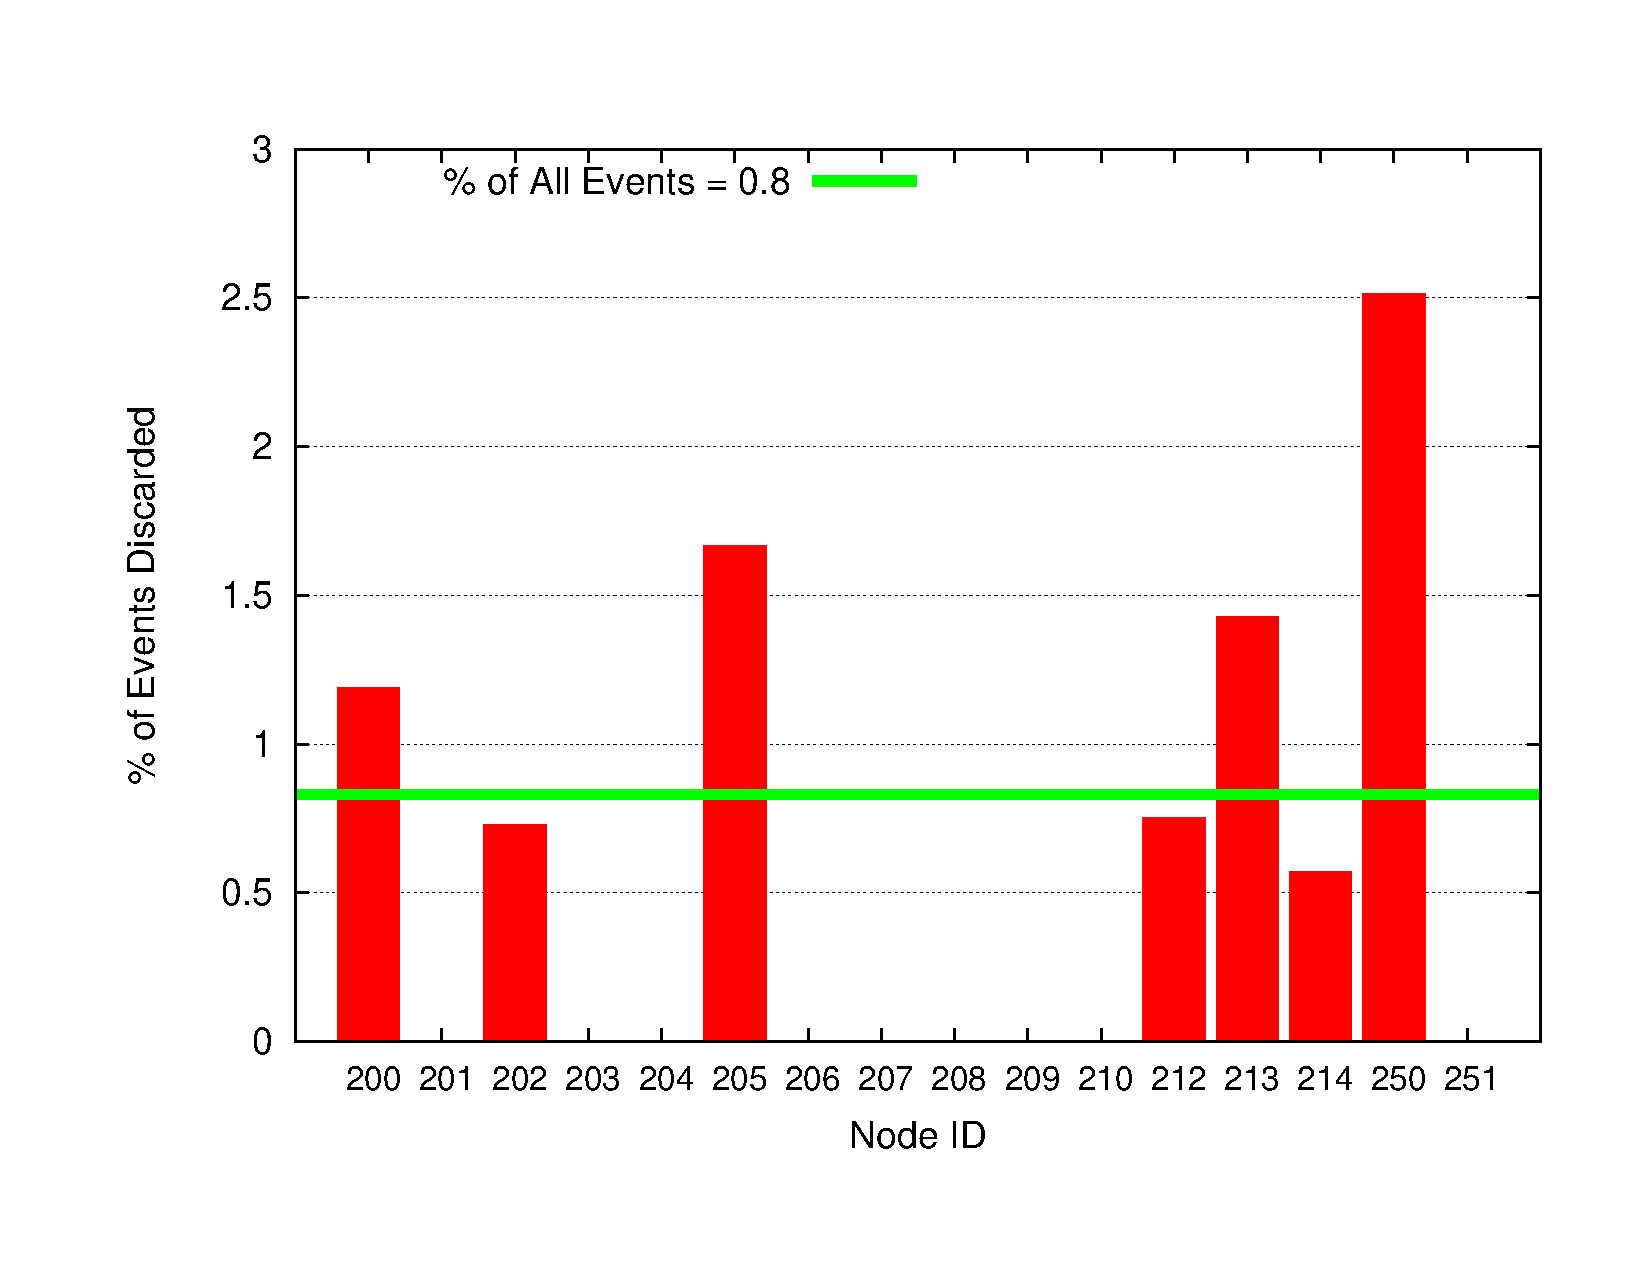
\includegraphics[width=\hsize]{./casestudy/figs/timing/TimingErrors/TIMINGFAILURES.pdf}
%\end{center}
%\caption{\small{\bf Percentage of Events Discarded Due to FTSP Failures}
%{\em For each node in the network this graphs shows the percentage of
%collected event records that were discarded due to bad FTSP timestamps. Node
%250 has the largest number of event records discards with around 2.5\%, which
%makes sense given that as shown in Figure~\ref{fig-ftspdown} Node 250
%returned an unusually large number of FTSP timestamps discarded by the
%heuristic filter. For all nodes our time rectification process was able to
%correct timestamps for data records that, if using FTSP alone, might have
%been unrecoverable. \GWAnote{Might we worth combining with the percentage of
%bad FTSP timestamps Figure to show the improvement!}}}
%\label{fig-timingfailures}
%\end{figure}

